\lstinputlisting[language=bash,basicstyle=\small]{python_codes/fieldstone_89/keywords}

\begin{center}
Code at \url{https://github.com/cedrict/fieldstone/tree/master/python_codes/fieldstone_89}
\end{center}

\par\noindent\rule{\textwidth}{0.4pt}

{\sl This stone was developed in collaboration wth Taco Broerse}. \index{contributors}{T. Broerse}

\par\noindent\rule{\textwidth}{0.4pt}

%%%%%%%%%%%%%%%%%%%%%%%%%%%%%%%%%%%%%%%%%%%%%%%%%%%%%%%%%%%%%%%%%%%%%%%%%%%%%%%%%%%%%%%%

The domain is a rectangle of size $L_x\times L_y$ discretised by nelx X nely Q2 elements..
The following velocity field is precribed in the domain:
\[
u(x,y)=0
\qquad
v(x,y)=A\;  \text{erf} (x-L_x/2)
\]
\begin{center}
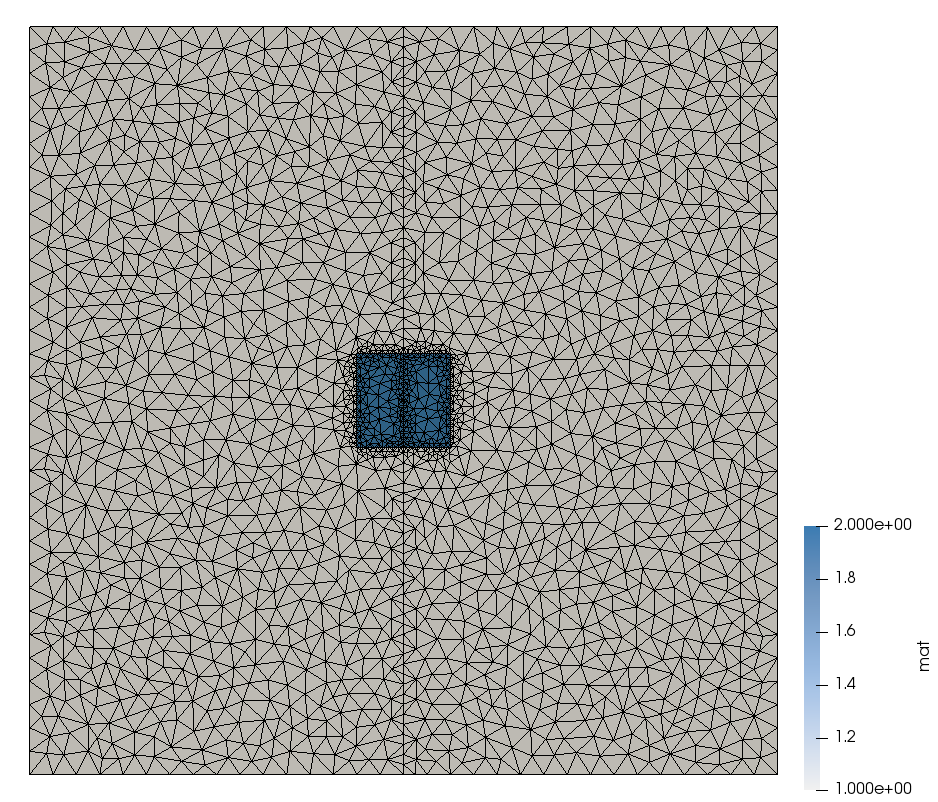
\includegraphics[width=6cm]{python_codes/fieldstone_89/images/grid}
\includegraphics[width=6cm]{python_codes/fieldstone_89/images/grid_vel}\\
{\captionfont Domain is 8x12, resolution 40x60. A=0.5}
\end{center}

A swarm of markers is then placed in the domain with about 9 markers per element, 
and they are then painted as shown here:
\begin{center}
\includegraphics[width=6cm]{python_codes/fieldstone_89/images/swarm_pos}
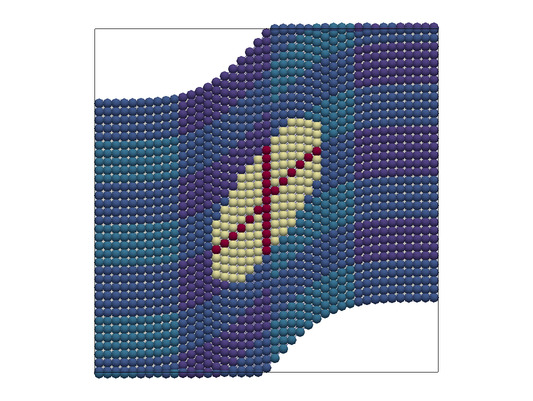
\includegraphics[width=6cm]{python_codes/fieldstone_89/images/swarm_paint}
\end{center}

A time loop is implemented. At each time step the velocity field of the grid is 
interpolated onto each marker that is in turn advected with a simple euler step. 
\[
\vec{x}(t+\delta t) = \vec{x}(t) + \vec\upnu \; \delta t
\]
Note that the timestep value $\delta t$ isc ontrolled by means of a CFL condition 
with ${\cal C}=0.1$. Likewise, the components of the strain rate tensor are computed on each marker and 
used to update the strain on each marker:
\[
\varepsilon_{ij}(t+\delta t) = \varepsilon_{ij}(t) + \dot\varepsilon_{ij}(t) \; \delta t
\]
These markers form a Lagrangian mesh which deforms over time:
\begin{center}
\includegraphics[width=6cm]{python_codes/fieldstone_89/images/swarm_mesh_later.png}
\includegraphics[width=6cm]{python_codes/fieldstone_89/images/swarm_paint_later}
\end{center}




-----------------------

\paragraph{Theory}


The current location $\vec{x}_i(t)$ of a marker $i$ at time $t$ that initially had the reference
position $\vec{X}$ is computed as follows:
\[
\vec{x}_i(t)= \vec{X}_i + \sum_{k=1}^{nstep}  \underbrace{\upnu(\vec{x}_i^k \; \delta t}_{\delta \vec{u}_i^k}
\]
where $\delta \vec{u}_i^k$ is the incremental Eulerian displacement at time $t=k\delta t$.
We obtain $\delta \vec{u}_i$ (we omit the $k$ upperscript from now on) through 
biquadratic interpolation of the velocity from the fixed Eulerian grid (the marker $i$
is first located in an element and shape functions are used).

From the Lagrangian positions in time we derive the deformation gradient F, that we will use
later to derive all deformation measures such as strain and stretch.
The deformation gradient relates initial vectors of the undeformed material
$d\vec{X}$ to the deformed, final material vector $d\vec{x}$, by
\[
d\vec{x} = {\bm F}\cdot d\vec{X}
\]
and this means that the deformation gradient tensor is defined as: 
\[
{\bm F} = \frac{\partial \vec{x}}{\partial \vec{X}}
\]
\index{general}{Deformation Gradient Tensor}

ABSORB fig 2 of Broerse

We can write the displacement u as the difference between current and reference coordinates:
\[
\vec{u} = \vec{x}-\vec{X}
\]
and the deformation gradient can be reformulated as a function of the displacements:
\[
{\bm F} 
= \frac{\partial \vec{x}}{\partial \vec{X}} 
= \frac{\partial }{\partial \vec{X}} (\vec{X}+\vec{u})
= {\bm I} + \frac{\partial \vec{u}}{\partial \vec{X}} 
= {\bm I} + \vec{\nabla}\vec{u} 
\]
From this it follows that the infinitesimal strain tensor can be written
\[
{\bm \varepsilon} = \frac{1}{2}( \vec\nabla\vec{u} + \vec\nabla\vec{u}^T )
= \frac{1}{2} (  {\bm F} +  {\bm F}^T) - {\bm I} 
\]
and the rotation tensor is then 
\[
{\bm \omega} 
=\frac{1}{2}( \vec\nabla\vec{u} - \vec\nabla\vec{u}^T )
= \frac{1}{2} (  {\bm F} -  {\bm F}^T)
\]


Any deformation that can be described by ${\bm F}$ 
can be written as a serial combination of a
simple shear, simple extensions along the x or y axes and a rotation:
\[
{\bm F} = {\bm Q} \cdot \tilde{\bm F}
\]
where $\tilde{\bm F}$ contains all shape changes and ${\bm Q}$ 
is an orthogonal rotation matrix (i.e. ${\bm Q}^T{\bm Q}={\bm I}$.
Furthermore, the distortion $\tilde{\bm F}$ can very conveniently be 
written as a successive multiplication of first a
shearing motion followed by a biaxial extension:
\[
\tilde{\bm F} 
= {\bm \Lambda} \cdot {\bm \Gamma }
=
\left(
\begin{array}{cc}
a & 0 \\ 0 & b 
\end{array}
\right)
\cdot
\left(
\begin{array}{cc}
1 & \gamma \\ 0 & 1 
\end{array}
\right)
=
\left(
\begin{array}{cc}
1 & a \gamma \\ 0 & b 
\end{array}
\right)
\]



\paragraph{Implementation}
The deformation gradient tensor is denoted ${\bm F}$ and is computed in the middle of
each cell at a fiven time $t$ as follows:
\[
{\bm F}(t)
=
\left(
\begin{array}{cc}
F_{xx} & F_{xy} \\
F_{yx} & F_{yy} 
\end{array}
\right)
=
{\bm I}+
\left(
\begin{array}{cc}
\frac{\partial (x(t)-x_0)}{\partial x}  & \frac{\partial (x(t)-x_0)}{\partial y}  \\
\frac{\partial (y(t)-y_0)}{\partial x}  & \frac{\partial (y(t)-y_0)}{\partial y}  
\end{array}
\right)
\]
In what follows we omit the time dependence '$(t)$'.
Each cell is assumed to be a $Q_1$ quadrilateral with a marker at each corner. We therefore store the 
initial position of markers, and make use of bilinear $Q_1$ shape functions to compute the derivatives
above in the center of the cell.


Since the centroids of the cells only move up, their $x$ position does not change 
at all, and then $x(t)-x_0=0$ and then $F_{xx}=1$ and $F_{xy}=0$.



\begin{enumerate}
\item The right Cauchy-Green deformation tensor is defined as
\[
{\bm C} = {\bm F}^T {\bm F}
\]
\item 
We then find the eigenvalues of ${\bm C}$:
\[
\mu_{1,2} = \frac{1}{2}(C_{xx}+C_{yy}) \pm \sqrt{ \frac{1}{4}(C_{xx}-C_{yy})^2 + C_{xy}^2   }
\]
\item We compute the two invariants:
\[
I_C = \mu_1+\mu_2 \qquad II_C = \mu_1\mu_2 
\]
\item Compute invariants of right stretch tensor U
\[
I_U=\sqrt{I_C+2\sqrt{II_C}}
\qquad
II_U=\sqrt{II_C}
\]
\item compute right stretch tensor ${\bm U}$
\[
{\bm U} = \frac{{\bm C}+ II_U {\bm I}}{I_U}
\]
\item compute inverse of ${\bm U}$
\[
{\bm U}^{-1} = - I_U \frac{{\bm C}- (II_U+I_C){\bm I}}{II_U(II_U+I_C)+II_C}
\]
\item compute rotation matrix ${\bm R}={\bm F}{\bm U}^{-1}$

\item compute left stretch tensor ${\bm V}={\bm F}{\bm R}^T$

\item Compute eigenvalues of ${\bm V}$, which are the square roots of those of ${\bm C}$
\[
\lambda_1 = \sqrt{\mu_1}
\qquad
\lambda_2 = \sqrt{\mu_2}
\]


\end{enumerate}



Message:
infinitesimal strains, or integrated strain rates lose their physical meaning when 
the deformation becomes large

What I/the community does wrong:
on markers, we interpolate grav v through Q1 fcts , we compute \dot{eps}_ij, we
update the starin as eps_ij += dot{eps}_ij . dt 
this is 'ok' only for (very) small total strains 
compare eigenvalues / principal strains eps_1, eps_2  


Malvern, then Taco have a better method to compute this total strain. 
We tesselate the marker swarm in quadrilaterals and we will compute
strain-related quantities in their centroids.

for each cell centroid, we compute the displacement gradient tensor F, 
then carry out polar decomposition to write F as product of stretch and rotation. 
F = R U  or F=  V R (we use the latter).
From V we compute the principal stretches (eigenvectors/values of V) bc
these represent the axes of the strain ellipse, i.e. directions of max stretch.
substract 1 to principal stretches to get principal strains, eps_1,2 = lamda_1,2 - 1,2 
compare these : the Malvern methid is supposefdly exact, so the difference tells me 
how bad my method is (up to few tens of \%) 
Also principal strains can never be smaller than -1 by def, because less than -1 means
more than 100\%  shortening (in 1D). but no upper limit.
conversely principal stretch > 0 (bc it is strain +1 ).







